\NeedsTeXFormat{LaTeX2e}
\documentclass[a4paper,12pt]{scrartcl}

%--------------------------------------------------------------------------

%Pakete
%------

\usepackage[utf8]{inputenc}
\usepackage{bookmark}
%Abbildungen
\usepackage{graphicx}
\usepackage{caption}
%Unterverzeichnis, in dem Abbildungen liegen
%\graphicspath{{figures/}}
%\usepackage{subfigure}
\usepackage{float}
%\usepackage{floatflt}
%schmalere Raender
\usepackage{a4wide}
%Formeln und Symbole
\usepackage{amsmath}
\usepackage{amstext}
\usepackage{amsfonts}
\usepackage{amsthm}
\usepackage{amssymb}
\usepackage{latexsym}
\usepackage{tikz}
\usepackage{setspace}
%Stichwortverzeichnis
%\usepackage{makeidx}
%Algorithmen darstellen
\usepackage[lined, shortend, linesnumbered]{algorithm2e} 
%deutsches Literaturverzeichnis
\usepackage{bibgerm}
%Textsprache deutsch
\usepackage[ngerman]{babel}
\usepackage[german]{varioref}
%mehrere Spalten
\usepackage{multicol}
%Links im Text
\usepackage{url}
\usepackage{hyperref}
%pdf-Seiten einbinden, wird für Eidesstattliche Versicherung benötigt
\usepackage{pdfpages}
\usepackage{listingsutf8}
\lstset{literate=%
    {Ö}{{\"O}}1
    {Ä}{{\"A}}1
    {Ü}{{\"U}}1
    {ß}{{\ss}}1
    {ü}{{\"u}}1
    {ä}{{\"a}}1
    {ö}{{\"o}}1
    {~}{{\textasciitilde}}1
}


 \begin{document}
Beim Papierflieger wird eine vorgefertigte Flugbahn durchflogen. Die vier verschiedenen
Flugbahnen sind in den unteren Abbildungen dargestellt. Hierbei wurde die Höhe (y-Koordinate) gegen
die Weite (x-Koordinate) angetragen, wodurch man die Seitenansicht der Flugbahn
sieht. Die verschiedenen Flugbahnen entstehen wie in Abschnitt 2.1 beschrieben durch
die unterschiedlichen Startwerte und ein Durchlauf entspricht dabei den Werten nach einem Zeitschritt (hier t=0.005s).  Die Flugbahnen mit Ausnahme von dem letzten Graphen sind glatte Funktionen, die stetig differenzierbar
sind und daher als sinnvolle Lösungen angesehen werden können.
Da der hier verwendete Löser dem Löser des Matlab-Originalcodes (ode23.m) entspricht
und nur minimale Rundungsfehler auftreten, stimmen die Ergebnisse des Matlab-Codes
(s.Tab. Originalcode) und unseres Codes (s.Tab. Eigencode) sehr gut überein. Dadurch gibt es auch im
Simulator keine größeren Fehler und der Flug sieht flüssig aus. \\
Im Fall des Gleitflugs (s.Abb.\ref{fig:gleit}) erkennt man, dass die prozentuale Abweichung in der Geschwindigkeit und im Steigungswinkel null beträgt. Dies kommt dadurch zu Stande, dass in diesem Fall der Winkel gesetzt wird und konstant bleibt, wodurch bei der Berechnung der Geschwindigkeit auch keine Abweichungen auftauchen. Allerdings ergeben sich Rundungsfehler bei der Höhe und der Weite, wobei der Fehler bei der Höhe mit jedem Durchlauf zunimmt, aber trotzdem nur bei 0.076\% nach 9 Durchläufen liegt. Die Abweichung bei der Weite ist aufgrund der niedrigen Werte höher, aber sie ist im Vergleich zur Höhe einigermaßen konstant und befindet sich im Bereich 5.2 - 5.7\%.\\
Wenn man sich nun den Sinusflug betrachtet (s.Abb.\ref{fig:sin}), erkennt man, dass die Abweichung bei der Weite wie beim Gleitflug verhält. Die Höhe hingegen ist bis auf zwei Werte absolut exakt, was mit dem niedrigen Steigungswinkel zusammenhängt. Dieser wiederum weist aufgrund der niedrigen Werte sehr starke Abweichungen auf, die sich dann in einem Bereich von 7 - 9\% einpendeln. Dadurch erhöht sich die Abweichung bei der Geschwindigkeit in jedem Zeitschritt, aber befindet sich noch deutlich unter 1\%. Wenn man nun beim Sinusflug die Geschwindigkeit weiter erhöhen würde wie in den nächsten beiden Fällen(s.Abb.\ref{fig:sin2} und \ref{fig:sin3}), würde man erkennen, dass sich die Geschwindigkeit und die Höhe wie zuvor mit wiederholter Durchführung zunehmend abweichen, aber immer noch eindeutig unter 1\% liegen. Die Abweichung in der Weite liegen auch wieder knapp über 5\% und der Steigungswinkel nähert sich auch der 5\%-Grenze an.\\
\begin{figure}[htp]
	\centering
	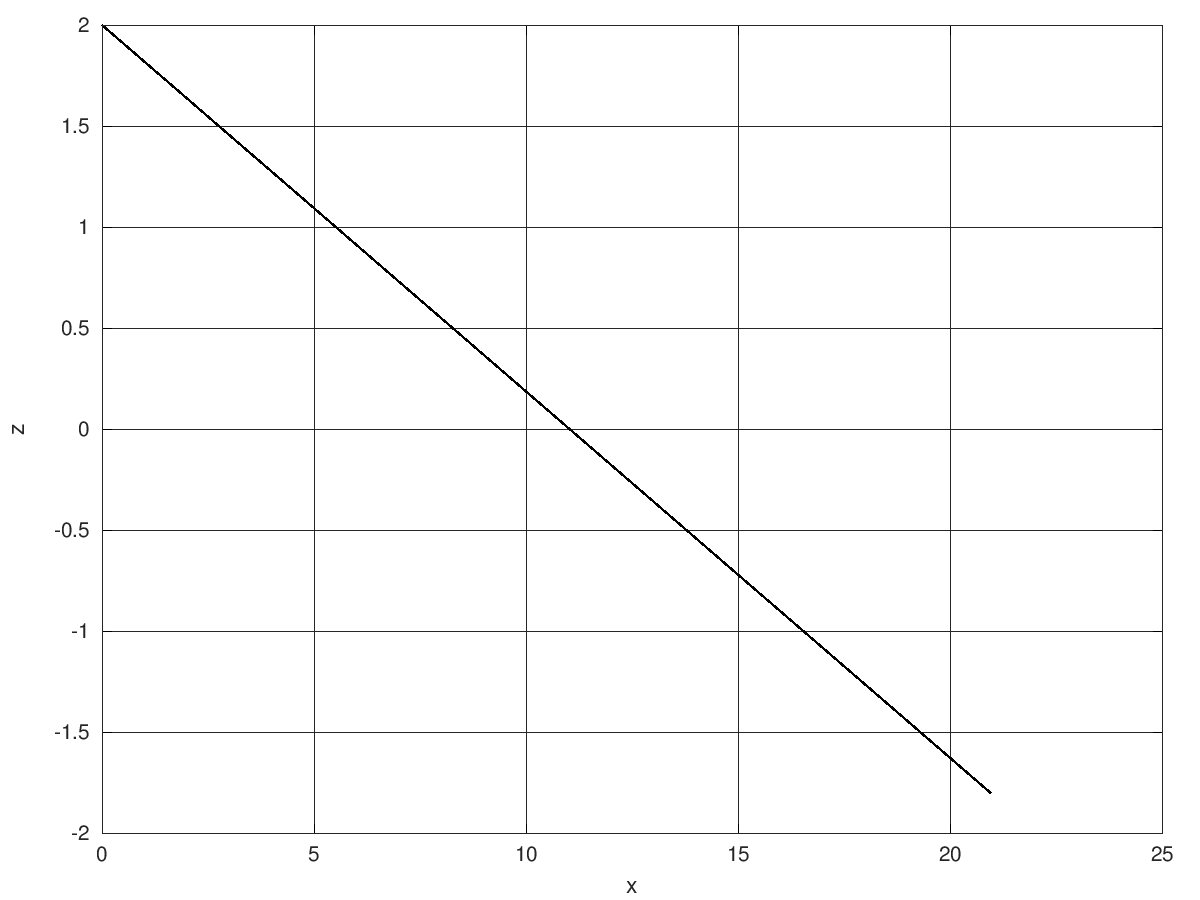
\includegraphics[width=300pt]{flightpath1.png}
	\captionof{figure}{Gleitflug}
	\label{fig:gleit}
\end{figure}
\begin{table}
\centering
\caption{Gleitflug - Eigencode}
\begin{tabular}{lllll}
Durchläufe & Geschw. & Steigungsw. & Höhe   & Weite   \\
1          & 3.5393  & -0.1794     & 1.9966 & 0.0184  \\
2          & 3.5393  & -0.1794     & 1.9933 & 0.0368  \\
3          & 3.5393  & -0.1794     & 1.9899 & 0.0552  \\
4          & 3.5393  & -0.1794     & 1.9866 & 0.0737  \\
5          & 3.5393  & -0.1794     & 1.9832 & 0.0921  \\
6          & 3.5393  & -0.1794     & 1.9799 & 0.1105  \\
7          & 3.5393  & -0.1794     & 1.9765 & 0.1290  \\
8          & 3.5393  & -0.1794     & 1.9732 & 0.1474  \\
9          & 3.5393  & -0.1794     & 1.9699 & 0.1658 
\end{tabular}
\end{table}
\begin{table}
\centering
\caption{Gleitflug - Originalcode}
\begin{tabular}{lllll}
Durchläufe & Geschw. & Steigungsw. & Höhe   & Weite   \\
1          & 3.5493  & -0.1794     & 1.9968 & 0.0174  \\
2          & 3.5493  & -0.1794     & 1.9936 & 0.0349  \\
3          & 3.5493  & -0.1794     & 1.9905 & 0.0523  \\
4          & 3.5493  & -0.1794     & 1.9873 & 0.0698  \\
5          & 3.5493  & -0.1794     & 1.9841 & 0.0873  \\
6          & 3.5493  & -0.1794     & 1.9810 & 0.1047  \\
7          & 3.5493  & -0.1794     & 1.9778 & 0.1222  \\
8          & 3.5493  & -0.1794     & 1.9746 & 0.1397  \\
9          & 3.5493  & -0.1794     & 1.9714 & 0.1571 
\end{tabular}
\end{table}
\begin{table}
\centering
\caption{Gleitflug - prozentuale Abweichungen}
\begin{tabular}{lllll}
Durchläufe & Geschw. & Steigungsw. & Höhe   & Weite   \\
1          & 0  & 0     & -0.0100 & +5.7471  \\
2          & 0  & 0     & -0.0150 & +5.4441  \\
3          & 0  & 0     & -0.0301 & +5.5449  \\
4          & 0  & 0     & -0.0352 & +5.5449  \\
5          & 0  & 0     & -0.0453 & +5.4982  \\
6          & 0  & 0     & -0.0555 & +5.5396  \\
7          & 0  & 0     & -0.0657 & +5.2713  \\
8          & 0  & 0     & -0.0709 & +5.5118  \\
9          & 0  & 0     & -0.0760 & +5.3469 
\end{tabular}
\end{table}
\begin{figure}[htp]
	\centering
	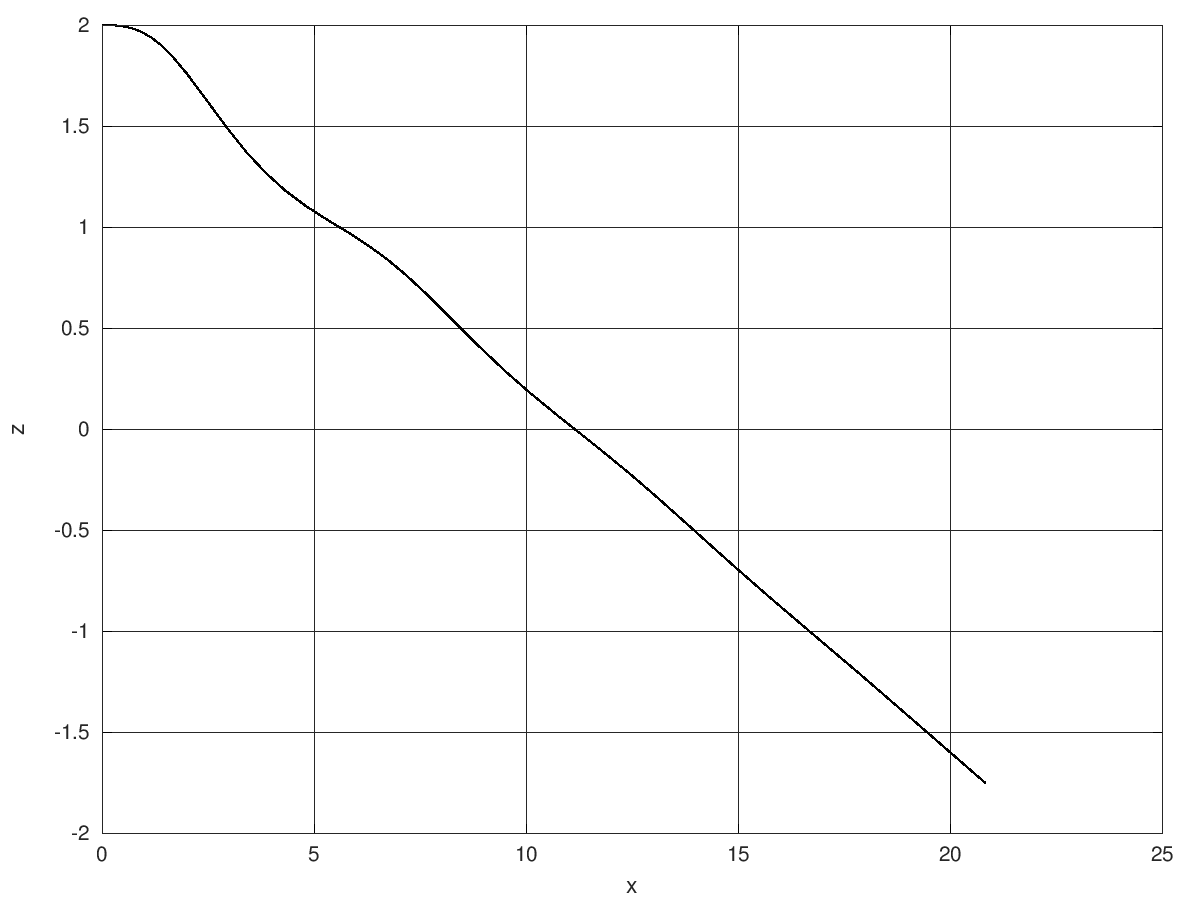
\includegraphics[width=300pt]{flightpath2.png}
	\captionof{figure}{Sinusflug}
	\label{fig:sin}
\end{figure}
\begin{table}
\centering
\caption{Sinusflug - Eigencode}
\begin{tabular}{lllll}
Durchläufe & Geschw. & Steigungsw. & Höhe   & Weite   \\
1          & 3.5401  & -0.0002     & 1.9999 & 0.0187  \\
2          & 3.5310  & -0.0006     & 1.9999 & 0.0373  \\
3          & 3.5219  & -0.0010     & 1.9999 & 0.0559  \\
4          & 3.5129  & -0.0015     & 1.9999 & 0.0745  \\
5          & 3.5040  & -0.0020     & 1.9999 & 0.0930  \\
6          & 3.4951  & -0.0027     & 1.9998 & 0.1115  \\
7          & 3.4864  & -0.0034     & 1.9998 & 0.1299  \\
8          & 3.4777  & -0.0042     & 1.9997 & 0.1483  \\
9          & 3.4691  & -0.0050     & 1.9996 & 0.1666 
\end{tabular}
\end{table}
\begin{table}
\centering
\caption{Sinusflug - Originalcode}
\begin{tabular}{lllll}
Durchläufe & Geschw. & Steigungsw. & Höhe   & Weite   \\
1          & 3.5406  & -0.0002     & 2.0000 & 0.0177  \\
2          & 3.5319  & -0.0005     & 1.9999 & 0.0354  \\
3          & 3.5233  & -0.0009     & 1.9999 & 0.0530  \\
4          & 3.5148  & -0.0014     & 1.9999 & 0.0706  \\
5          & 3.5063  & -0.0019     & 1.9999 & 0.0881  \\
6          & 3.4979  & -0.0025     & 1.9998 & 0.1057  \\
7          & 3.4896  & -0.0031     & 1.9998 & 0.1231  \\
8          & 3.4813  & -0.0039     & 1.9997 & 0.1406  \\
9          & 3.4732  & -0.0046     & 1.9997 & 0.1579 
\end{tabular}
\end{table}
\begin{table}
\centering
\caption{Sinusflug - prozentuale Abweichungen}
\begin{tabular}{lllll}
Durchläufe & Geschw. & Steigungsw. & Höhe   & Weite   \\
1          & -0.0141  &  0    & -0.0050 & +5.6497   \\
2          & -0.0254  &  -20    & 0 & +5.3672  \\
3          & -0.0397  &  -10    & 0 &  +5.4716 \\
4          & -0.0540  &   -7.1428   & 0 & +5.5240  \\
5          & -0.0655  &   -5.2631   & 0 &  +5.5618 \\
6          & -0.0800  &   -7.4074   &  0&   +5.4872\\
7          & -0.0917  &   -9.6774   &  0&   +5.5239\\
8          & -0.1034  &   -7.6923   &  0&   +5.4765\\
9          & -0.1698  &   -8.6956   & -0.0050 &  +5.5098
\end{tabular}
\end{table}
\begin{figure}[htp]
	\centering
	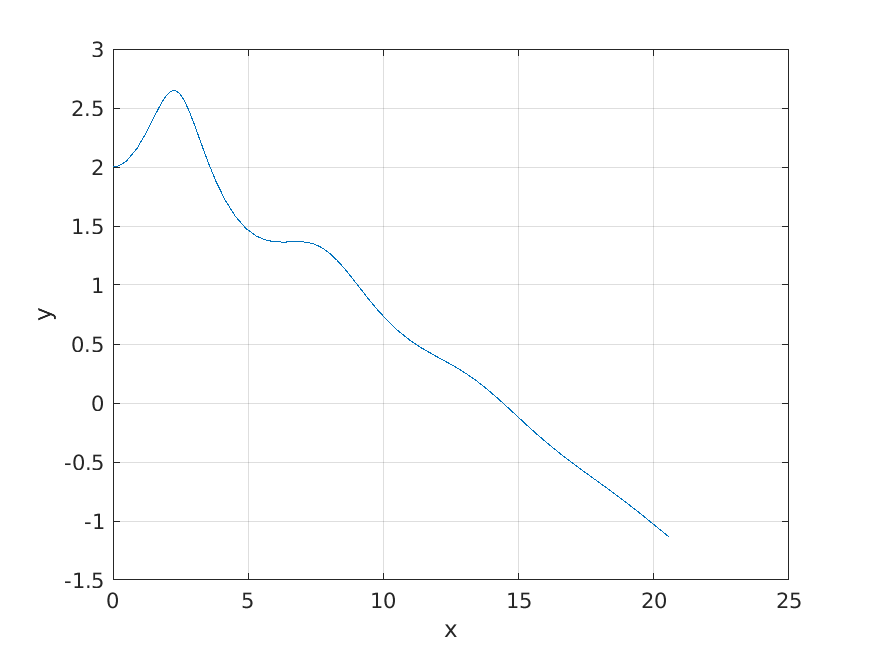
\includegraphics[width=300pt]{flightpath3.png}
	\captionof{figure}{Sinusflug mit erhöhter Geschwindigkeit}
	\label{fig:sin2}
\end{figure}
\begin{table}
\centering
\caption{Sinusflug mit erhöhter Geschwindigkeit - Eigencode}
\begin{tabular}{lllll}
Durchläufe & Geschw. & Steigungsw. & Höhe   & Weite    \\
1          & 5.3030  & 0.0117      & 2.0001 & 0.0280   \\
2          & 5.2816  & 0.0233      & 2.0006 & 0.0559   \\
3          & 5.2597  & 0.0348      & 2.0014 & 0.0837  \\
4          & 5.2374  & 0.0461      & 2.0025 & 0.1114   \\
5          & 5.2147  & 0.0574      & 2.0040 & 0.1390   \\
6          & 5.1916  & 0.0685      & 2.0057 & 0.1664   \\
7          & 5.1681  & 0.0795      & 2.0077 & 0.1936   \\
8          & 5.1443  & 0.0903      & 2.0100 & 0.2207   \\
9          & 5.1200  & 0.1010      & 2.0126 & 0.2477  
\end{tabular}
\end{table}
\begin{figure}[htp]
	\centering
	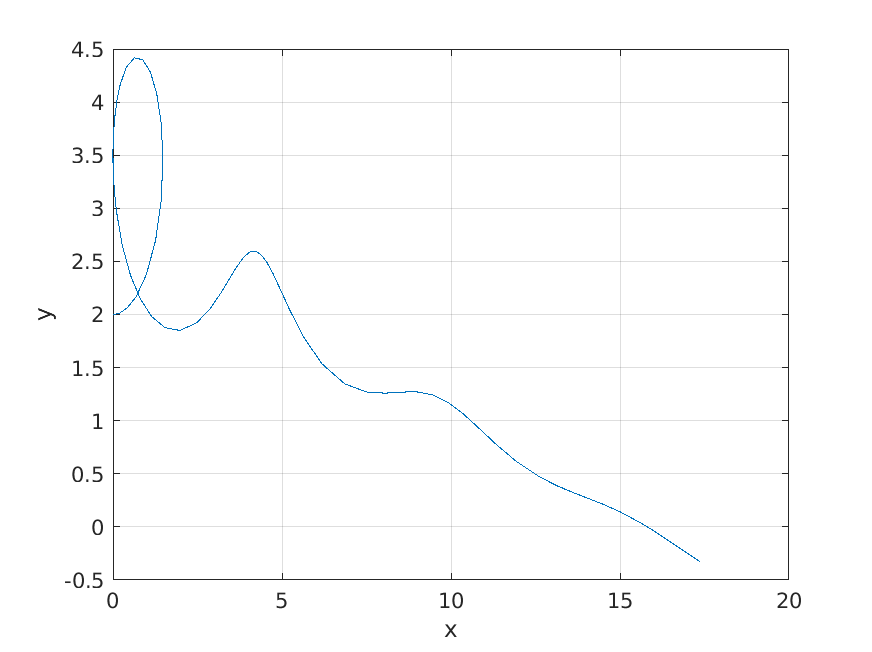
\includegraphics[width=300pt]{flightpath4.png}
	\captionof{figure}{Sinusflug mit weiter erhöhter Geschwindigkeit}
	\label{fig:sin3}
\end{figure}
\begin{table}
\centering
\caption{Sinusflug mit erhöhter Geschwindigkeit - Originalcode}
\begin{tabular}{lllll}
Durchläufe & Geschw. & Steigungsw. & Höhe    & Weite    \\
1          & 5.3041 & 0.0111     & 2.0001 & 0.0265  \\
2          & 5.2839 & 0.0221     & 2.0005 & 0.0530  \\
3          & 5.2632 & 0.0330     & 2.0013 & 0.0793  \\
4          & 5.2422 & 0.0438     & 2.0023 & 0.1056  \\
5          & 5.2208 & 0.0544     & 2.0036 & 0.1317  \\
6          & 5.1990 & 0.0650     & 2.0051 & 0.1577  \\
7          & 5.1769 & 0.0754     & 2.0069 & 0.1836  \\
8          & 5.1544 & 0.0857     & 2.0090 & 0.2093  \\
9          & 5.1316 & 0.0959     & 2.0114 & 0.2350 
\end{tabular}
\end{table}
\begin{table}
\centering
\caption{Sinusflug mit weiter erhöhter Geschwindigkeit -  Eigencode}
\begin{tabular}{lllll}
Durchläufe & Geschw. & Steigungsw. & Höhe   & Weite   \\
1          & 10.5646 & 0.0379      & 2.0010 & 0.0559  \\
2          & 10.4805 & 0.0756      & 2.0042 & 0.1114  \\
3          & 10.3958 & 0.1128      & 2.0093 & 0.1662  \\
4          & 10.3104 & 0.1497      & 2.0165 & 0.2204  \\
5          & 10.2245 & 0.1862      & 2.0256 & 0.2738  \\
6          & 10.1380 & 0.2224      & 2.0365 & 0.3264  \\
7          & 10.0510 & 0.2582      & 2.0492 & 0.3782  \\
8          & 9.9635  & 0.2937      & 2.0635 & 0.4290  \\
9          & 9.8755  & 0.3288      & 2.0796 & 0.4788 
\end{tabular}
\end{table}
\begin{table}
\centering
\caption{Sinusflug mit weiter erhöhter Geschwindigkeit - Originalcode}
\begin{tabular}{lllll}
Durchläufe & Geschw.  & Steigungsw. & Höhe   & Weite      \\
1          & 10.5691 & 0.0359     & 2.0009 &  0.0530  \\
2          & 10.4895 & 0.0716     & 2.0037 &  0.1056  \\
3          & 10.4093 & 0.1069     & 2.0084 &  0.1576  \\
4          & 10.3286 & 0.1419     & 2.0148 &  0.2090  \\
5          & 10.2473 & 0.1766     & 2.0230 &  0.2598  \\
6          & 10.1656 & 0.2109     & 2.0328 &  0.3099  \\
7          & 10.0833 & 0.2450     & 2.0443 &  0.3592  \\
8          & 10.0007 & 0.2787     & 2.0573 &  0.4077  \\
9          & 9.9175 & 0.3121     & 2.0718 &  0.4553 
\end{tabular}
\end{table}
\newpage
Beim echten Flugzeug wurde, wie in Abschnitt 2.2 beschrieben, ein expliziter Löser verwendet,
wobei im Matlab-Originalcode ein impliziter Löser (ode15s.m) verwendet wurde.
Unser Löser bietet eine gute Näherung, entspricht den Daten aus dem Original-Code aber
nicht immer exakt. Daher kann unser Löser die Bewegungsgleichungen zu bestimmten
Eingabedaten nicht mehr lösen, da die Daten im Löser zu extrem großen Werten führen.
Der Löser funktioniert zu realistischen Eingabedaten aber sehr gut und ist außerdem
sehr effizient, was bei der Echtzeitlösung eine sehr große Rolle spielt. Deshalb ist auch
hier der Flug überwiegend flüssig, bis auf ein paar wenige Momente, wo selbst der explizite
Löser zu kleineren Fehlern führen kann.\\
Beim echten Flugzeug wurden zwei Fälle besonders analysiert, ein Kurvenflug und ein Sinusflug.
Hierbei entspricht ein Durchlauf bzw. Zeitschritt 1s. 
Beim Kurvenflug wurde anfangs das Querruder auf \(10^\circ\) eingestellt. Dadurch durch fliegt
das Flugzeug solange eine Linkskurve, bis der Benutzer per Steuerung das Querruder
wieder verstellt. Beim Betrachten der Flugbahn(s.Abb. \ref{fig:k1},\ref{fig:k2},\ref{fig:k3},\ref{fig:k4}) erkennt man, dass die Funktionen wie zuvor auch beim Papierflieger glatt sind, aber hier ist zu beachten, dass die Kurven nicht den originalen Kurven entsprechen, was durch den unterschiedlichen Löser zu Stande kommt. Trotzdem sind die Flugbahnen aufgrund der Glattheit und stetigen Differenzierbarkeit sinnvolle Lösungen.
\begin{figure}[htp]
	\centering
	\includegraphics[width=300pt]{kurve1.jpg}
	\captionof{figure}{Flugbahn im dreidimensionalen Koordinatensystem}
	\label{fig:k1}
\end{figure}
\begin{figure}[htp]
	\centering
	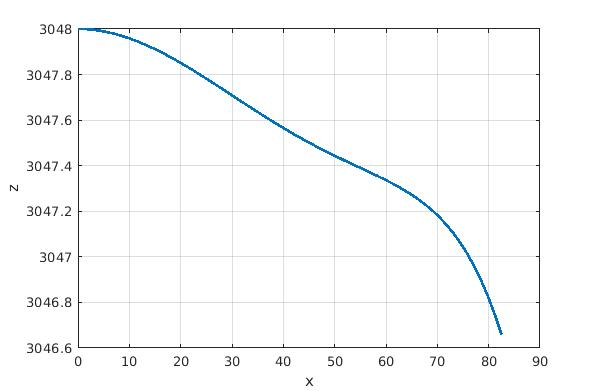
\includegraphics[width=300pt]{Kurve2.jpg}
	\captionof{figure}{Flugbahn in xz-Richtung}
	\label{fig:k2}
\end{figure}
\begin{figure}[htp]
	\centering
	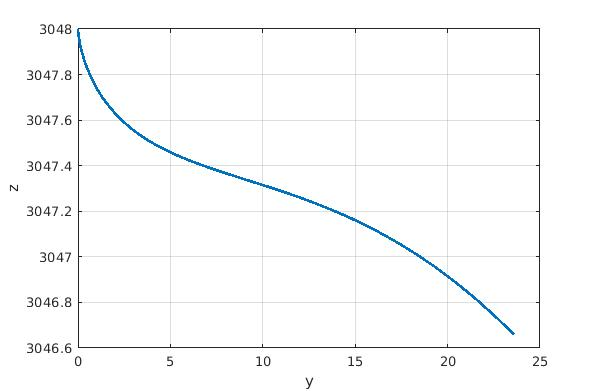
\includegraphics[width=300pt]{Kurve3.jpg}
	\captionof{figure}{Flugbahn in yz-Richtung}
	\label{fig:k3}
\end{figure}
\begin{figure}[htp]
	\centering
	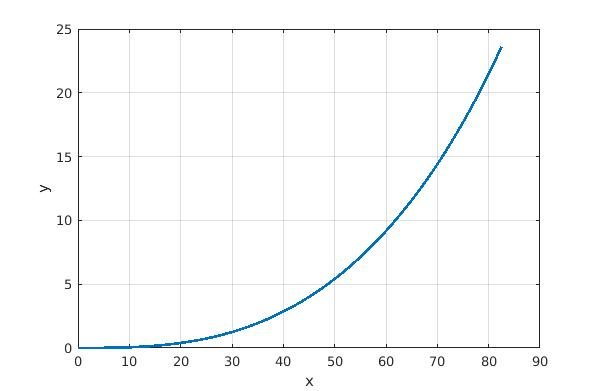
\includegraphics[width=300pt]{Kurve4.jpg}
	\captionof{figure}{Flugbahn in xy-Richtung}
	\label{fig:k4}
\end{figure}
\begin{table}
\centering
\caption{Kurvenflug}
\begin{tabular}{lllllll}
Durchläufe & x-Geschw. & z-Geschw. & y-Geschw. & Rollwinkel & Steigungsw. & Gierwinkel  \\
1          & 84.0979   & 30.1265   & 3.2128    & -0.0543    & -0.0326     & -0.3484     \\
2          & 75.0155   & 40.7627   & 10.5361   & -0.6684    & -0.2488     & -0.5803     \\
3          & 80.4611   & 24.3552   & -1.7105   & -1.4873    & -0.4077     & -0.2236     \\
4          & 82.8233   & 18.0573   & -1.5254   & -1.9282    & -0.4339     & -0.1027     \\
5          & 81.7825   & 27.8673   & 1.9416    & -2.3095    & -0.6482     & 0.0008      \\
6          & 81.6360   & 33.8844   & 3.0865    & -2.9630    & -0.7160     & 0.2154      \\
7          & 86.8729   & 29.7514   & 0.1934    & -3.5393    & -0.6131     & 0.2021      \\
8          & 92.3379   & 27.8664   & 0.1502    & -3.9942    & -0.5808     & 0.1271      \\
9          & 95.7539   & 32.8952   & 2.1490    & -4.4660    & -0.5373     & 0.0956     
\end{tabular}
\end{table}
\newpage
Beim Sinusflug wird der Schräglaufwinkel (sideslip angle) \(\beta\) beispielsweise auf \(80^\circ\) eingestellt, wodurch es
zur Side Force kommt. Man kann gut beobachten, wie das Flugzeug anfangs durch diese
seitliche Kraft kurz ins Schwanken gerät und dann wieder in den Geradeausflug zurück
kehrt. Dieser Effekt resultiert daraus, dass das Flugzeug aerodynamisch stabil gebaut ist.
 \end{document}.